\chapter{Test}\label{ch:test}
The primary test purpose is to reveal the presence of faults in a system. The main idea behind testing consists in applying test data to inputs of the IC, design, wafer, dice, or any other system called Unit Under Test (UUT) and collecting data from its outputs. The test data applied to the inputs is called the test vector or test stimuli and the data collected from the outputs - the response of the UUT. The term test pattern is used to describe the test vectors together with expected correct responses. A test set relates to a series of test patterns. After applying test vectors and capturing the responses, they are compared with a fault free response stored in the test pattern. If they differ in any position or value, fault is uncovered. The \autoref{fig:test} shows the typical test environment

\begin{figure}[H]
\centering
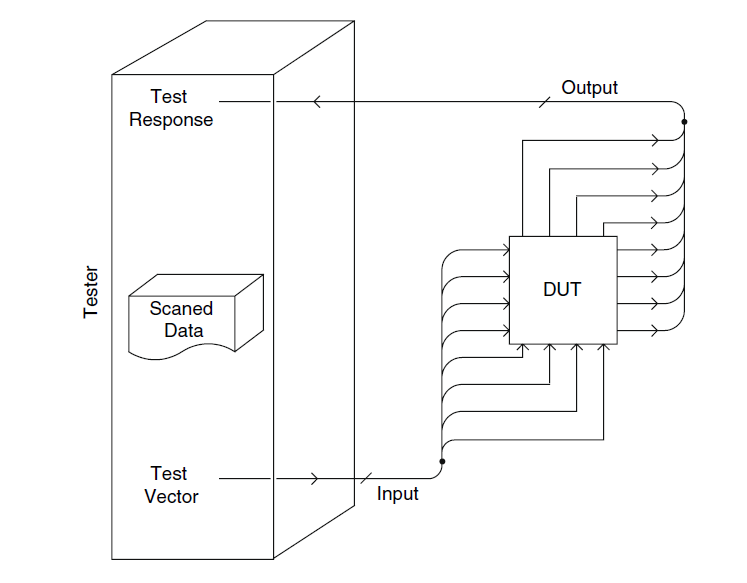
\includegraphics[width=0.65\textwidth]{figures/test.png}
\caption{The tester principle~\cite{book:Navabi}}
\label{fig:test}
\end{figure}


\section{Fault models}

While it is possible to prove the presence of faults in the design, there is no method proving their absence. The amount of different faults and their variety is countless, hence there are means needed to model how those faults affect the system. The fault itself is not visible to the tester itself (except from visual tests) and has to be stimulated to manifest, and in best case, propagate to the UUT outputs. Many different faults can have the same effect, so investigating the effects of faults may bring better results. The fault effects are called failure modes and they have to be modeled in order to conduct tests. Such fault models serve the purpose of altering the data flow, in the similar way, as the real faults would. It allows to develop test vectors to stimulate and propagate the real faults effects. There are two groups of fault models. The ones that describe faults affecting the logical operations and ones describing the defects in parameters. The most common logical fault models are:
\begin{itemize}
    \item Stuck-At-Fault consists in an assumption that a node in the design has a permanent value and doesn't respond to the logical transitions forced on it. The node can be Stuck-at-0 (SA0) or Stuck-at-1 (SA1)
    \item Bridging fault assumes that two nodes interact with each other unintentionally producing either a Wired-AND effect with 0-dominant connection or Wired-OR effect being 1 dominant.
    \item Delay fault may be considered as a parametric fault rather than a logic fault. The net delay fault occurs when a signal needs more time, to cover certain logical path, then assumed. The transmission delay faults describe the situtation when the fault is caused by fall and rise times of clock signal driving the logical gate, when the signal doesn't make it from the input to the output during one clock cycle. The result may be the previous value processed by consecutive gates or delayed value stored in a memory cell.
    \item Memory fault (logical faults considered)
    \item Single Event Transient (SET) describes a glitch in combinational logic that travels trough design.
    \item Single Event Upset (SEU) describes the situation when the incorrect voltage level caused by SET gets stored in the memory or the memory state changes. Can affect more memory cells at once.
    \item Single Event Latchup (SEL) - a highly loaded particle makes a locked transistor conduct leading to short in CMOS logic. Requires a power reset and may lead to a hard fault, because of a very high temperature~\cite{report:altera}.
\end{itemize}
The parametric faults are modeled through:
\begin{itemize}
    \item Bridging fault assumes resistive unintentional connection between two nodes
    \item Memory fault (non-logical faults considered)
    \item Open-circuit fault in interconnect metal
    \item Stuck-open and stuck-short faults in transistors
    \item $I_{DDQ}$ Fault - measuring the current by power supply during static operation of the design (while there is no switching activity)
\end{itemize}
All mentioned models represent failure modes in digital hardware logic, even the analog or mixed signal tests consider only digital circuits. Most operations however take less time and energy when moved from digital domain to analog one. Additionally every radio related circuit does some, or even majority of operations in analog domain and mixed-signal domain. In modern communication systems, with SoC technology, there is a rapid growth in analog and mixed circuitry that is also vulnerable to faults. The number of such faults is again countless and some sort of abstraction is required. The continuous characteristic of analog systems allows only for two fault models:
\begin{itemize}
    \item Catastrophic failures - the system is not functional at all
    \item Unacceptable performance - the service is still provided but some of the functionality lies outside of the acceptable range of the specification
\end{itemize}
The border line between those two is obviously very subjective and bases on the definition of system correct functionality.~\cite{book:Kabisatpathy}.
\section{Test Types}
Testing can be done in following ways:
\begin{itemize}
    \item External testing is when the design is tested by some external circuit from the tested design perspective. The internal testing assumes that all needed components are integrated in the circuit, like in case of the Built In Self Test described later.
    \item Online testing doesn't disturb hardwares normal operation, while an offline test requires the system to stop working for the test to be carried out.
    \item Concurrent testing is online testing that is carried out with normal data sets while normal system function.
    \item At-speed testing is conducted at normal speed of the design instead of lowered frequency, that needs to be specially generated for test purpose. To realize at-speed testing often a second, shifted frequency is required.
    \item Diagnostic test is carried out to find a cause of a failure
\end{itemize}

\section{Design For Testability (DfT)}
If the test vectors can only be applied to the unit inputs and responses sampled only from the outputs, many problems occur. While testing, the combinational fan-outs and reconvergences become problems. To stimulate faults laying deep inside the combinational logic structure, the test designer has to come up with such a vector, that will force a certain state in the logic and let this state propagate to one of the design outputs. Testing sequential logic in this way would be nearly impossible because of the complexity of creating and testing all possible states of such system. Therefore the testability has to be supported by system designers to allow test access to those parts of the design, that are difficult to test using only primary inputs and outputs. Incorporating the testability methods in the design work flow is called the Design For Testability and is a standard approach during the development of todays complex electronic systems. The designers have many options in making their designs easier to test, therefore maximizing the test coverage. Ease of test is meant both by reduced complexity of test and by easier physical access to the system. The means for testability are listed below.
\subsection{System Partitioning}
To increase testability the untestable complex systems have to be split into smaller testable units. If one wanted to test a 64-bits counter and compare each time against correct data, the test could take years. Splitting the counter into 4 16-bit counters reduces the test time to nearly half of a second. The tester has to deal with just 4 16 bit counters, that can be tested in parallel which would be impossible with one big counter.

Another example of partitioning is based on the knowledge how the sequential logic is built. Synchronous sequential systems can be represented as combinational logic with delayed feedback. The delay is implemented as flip-flops which separate the actual state of the system from its next state. The whole system can be therefore understood as the Meely state machine and is shown in the \autoref{fig:Meely}. Most of the logic gates reside in the combinational part, so the test procedure should focus on this part. Gaining access to present state inputs, together with manipulating the primary inputs, would allow the tester to determine an exact state of the system and test it.

\begin{figure}[H]
\centering
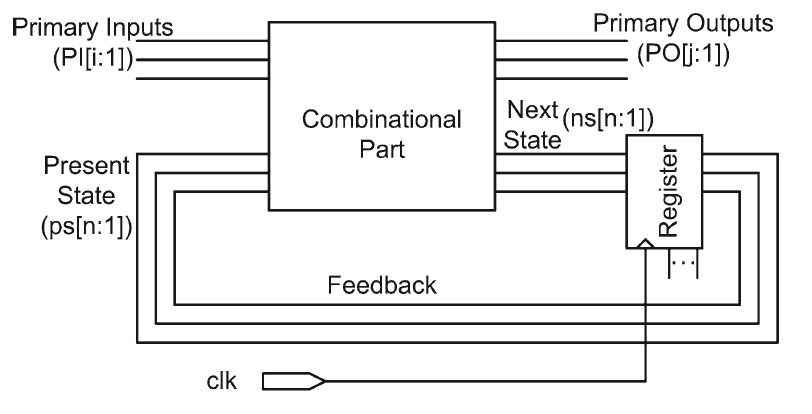
\includegraphics[width=0.65\textwidth]{figures/Meely.PNG}
\caption{Representation of a sequential system as the Meely state machine \cite{book:Navabi}}
\label{fig:Meely}
\end{figure}

\subsection{Scan test}
The "divide and conquer" approach allows other widely used methods to be implemented. The most common and supported method is a scan test. It exploits the method of unfolding the sequential logic into combinational part and memory feedback part. The flip-flops containing the present state of the system on their outputs and the next state of the system on their inputs are transformed into one big shift register. In normal mode the shift register is treated as parallel input parallel output register, with shifting option disabled. When the test takes place, the data is serially shifted through the shift register until all registers reach their determined state. The data is then shifted out for comparison. The shifting can be clocked with much higher frequency then the system is designed for, because until all registers are filled with data, the output of the combinational logic is irrelevant. The fast clocking can however lead to abnormal power consumption and heat emission and in result to systems premature deterioration. The test parameters have to be adjusted with care. The scan test is a crucial part of boundary scan technology, where scan path can be accessed as IO of the IC. The test pattern generation and response analysis is usually placed externally from the UUT and used only during the test procedure, for example during the post-manufacturing tests. The tools for pattern generation and response analysis are named Automatic Test Equipment (ATE) and can be dedicated to one chip or universally adaptable to test many different architectures. The configurable solution lowers the test costs and development time. Placing the test logic outside of the chip simplifies its design and lowers the complexity of the system.

\subsection{Buit-In-Self-Test (BIST)}
The test access to the IC is not only relevant during a post manufacture testing and should be possible not only with use of ATE. Many safety-critical or mission-critical applications require the unit to be able to conduct a local self tests autonomously and detect its own errors. The integration of test logic in the chip itself can also speed up the test process. The test equipment would only start the test routine and read the outcome. The Built-In-Self-Test consists of scan path, test pattern generator and output response analyzer integrated into the design. The test pattern generation is often conducted with the use of LFSR and its pseudo-random output. The patterns may also be stored in a ROM in a compressed form. The output response analyzer can compare either the whole input bit stream or just the signature of the response, in hope that they are different from the pre-calculated, fault-free signature. This approach may lead to undetected faults in cases of collisions in the signature generation algorithm.


\subsection{Analog and Mixed-Signal DfT}\label{sub:testa}
Together with the todays trend of integrating digital, analog and mixed-signal logic into one System-On-The-Chip (SoC), the external test of non-digital parts of the design is no longer sufficient. The mixed circuitry gets also widely implemented into safety- and mission-critical applications and requires appropriate DfT techniques.

The main drawback in adopting standard DfT techniques into an analog domain is the degradation of the signal quality, when any additional circuitry is being added to the signal paths. There is a mixed-signal test bus standard (IEEE Std 1149.4-1999) which provides a boundary scan capability, improving the controllability and observability of the design, but leaving the response analysis and wave generation to the ATE. Another problem is the not-ideal response of switches, which can distort the signal even when in normal mode.

There is no standardization of BIST techniques and most of the implementation tend to be ad-hoc. The on-chip analog test pattern generation has been proven to work with the use of Pulse Density Modulated signals, followed by low pass filters to create a wave of desired shape. The more "ones" following each other, the higher the amplitude of the output signal. The PDM signal is digitally generated and the response can be sampled back into the digital domain for comparison or evaluation. The sampling is possible thanks to the Delta-Sigma Modulator ($\Delta \Sigma M$), which recreates the digital bit stream with the density of ones proportional to the analog signal~\cite{book:Grout}.

The response analysis is another demanding task, usually done externally by ATE, together with sampling the output voltage and currents. With use of the Delta-Sigma Modulator or another ADCs, the analog signals can be evaluated as digital bit streams. The latest development in machine learning technologies proved to be successful in evaluation of many voltage levels coming from an RF chip and classifying them as faulty or fault-free~\cite{art:neural}.

\section{DfT Techniques in Encoders and Decoders}

As mentioned in \autoref{sec:Hsiao}, the SEC-DED codes are very fast, usually operate within one clock cycle but their main disadvantage are miscorrections of triple and multiple bit errors. Every transient or permanent fault in the encoder or decoder results in possible miscorrection. A single bit error due to a single fault in encoder gets detected and corrected by the decoder, but with simultaneous occurrence of a transmission error, the hardware fault stripped the system down from its correcting capabilities. In case of double bit error, together with hardware fault, a miscorrection is very probable. The same applies for decoder. A single error due to hardware fault in its embedded encoder will have the same effect as a single transmission error or an error in transmitters encoder. An error in syndrome calculation may also lead to a miscorrection. Moreover in the presented Hsiao encoder, every user bit takes part in building of three check bits, so any hardware fault in i.e its input registers may lead to a triple bit error, which will not get corrected by the decoder. Additionally every pair of user bits takes part in creation of two check bits. It means, that an output of a XOR operations feeds two subsequent operations. Big fan-outs also allow single faults to cause multiple bit errors. Luckily any particle causing a SET in combinational logic will result only in a "glitch", since the connection to the GND or VDD will quickly recover its correct state. In worst case a SET of a single gate output, causing a "glitch" in subsequent gates, gets stored in the output registers before the recovery. There are two approaches to counteract this behavior. The first possibility is to add more gates, to avoid big fan-outs and minimize the damage caused by any SET to one erroneous check bit. The other possibility is to protect the registers from transient faults and filter the combinational glitches with Muller-C elements at the same time\cite{art:Dicorato}.

The Muller-C element with two inputs, holds the last common input state at its output. Any change of one of its inputs doesn't change its output state. Both inputs need to change, to reload the output state. To filter the combinational glitches, a delay needs to be applied to one of the input flip-flops. The length of the delay will define the length of the glitch that may get filtered. This solution will not wowrk for longer SET or SEU or permanent faults in flip-flops \cite{art:Dicorato}.

To cope with permanent faults, another techniques need to be incorporated. The additional logic to avoid big XOR fan-outs made the system more regular. In regular systems, where some of the logic is simply multiplied and used in parallel, a simple duplication of any repeatable part gives the ability to conduct a test to uncover permanent faults. The reexecution on different units and comparison will show if any unit is faulty and will allow a repair, since the additional logic can be used as a spare. In less regular hardware, the duplication of bigger groups is necessary. It is estimated that the overhead for control logic and switches pays off for repeatable units over 300 transistors \cite{rescue_conference}. This solution works for offline error detection and self repair. To achieve online error correction and masking of permanent faults with the ability of repair during scheduled break or start up, a triplication in hardware is needed. Every repair procedure requires advanced clock control and additional time.

The decoders are circuits that can correct their own errors and errors of encoders in transmitter modules. Every error happening in the embedded encoder of the decoder will not be distinguished from any error that appeared in the transmitters encoder or on the transmission path. If the design is implemented according to proposed DfT techniques then any single transient fault in the embedded encoder will result in single error, which can be easily corrected by the decoder. For multiple error correction decoder, this acceptance is even higher. Only the accumulation of transmission and internal decoder and encoder faults that exceeds the decoder correction capabilities may lead to miscorrection, and in result to system failure. The proposed techniques don't cover however the syndrome calculation and therefore error location circuits. But again, the failure of one syndrome calculation may not lead to the system failure or even to the miscorrection. In the presented decoder, the single syndrome failure is 



\section{Functional Shorts Concept}\label{sec:shorts}
The hard errors due to permanent faults in hardware modules require special treatment since they can even prevent the synchronization of transceiver and receiver and therefore cannot be so easily corrected by FEC. Since permanent faults don't disappear, they also need special repair mechanism, which often means a doubling of the unit or its parts. The fault diagnosis proves to be complicated, especially in the mixed signal and analog parts, moreover when the access to this parts is limited. When an IP is shipped as a "black box" and there is no possibility to implement any internal DfT techniques, some sort of external test is required. 

Thanks to the ECC, a precise detection of error positions in the received bit stream is possible, as long as the error count doesn't exceed ECCs correcting capabilities. The idea behind the diagnostic test based on extended FEC functions is to use the existing FEC redundancy and detect not only soft errors and transmission errors, but also hard errors due to permanent faults. As mentioned in the~\autoref{sub:limits} the ECC can be used in hardware monitoring only if the input and output of the UUT are identical. Since the wireless communication is usually a duplex communication, every node happens to own both, the transmitter and receiver. They consist of complementary building blocks. Every modulator in transmitter is substituted with a demodulator in receiver, every encoder with decoder. The basic task of the receiver modules is to recreate the original information sent by transmitter, step by step, layer by layer. A diagnostic test would require to short the transmitter with receiver and systematically short the outputs of every module with the inputs of their corresponding module. With encoder and decoder in one closed system, it should be possible to detect the exact positions of errors in the bitstream and identify faulty units. The decoder would act as a response analyzer. In this way, the information leaving FEC encoder arrives at the input of FEC decoder, manipulated only by permanent faults in the shorted modules. The idea is presented in~\autoref{fig:Shorts}. 

\begin{figure}[h]
\centering
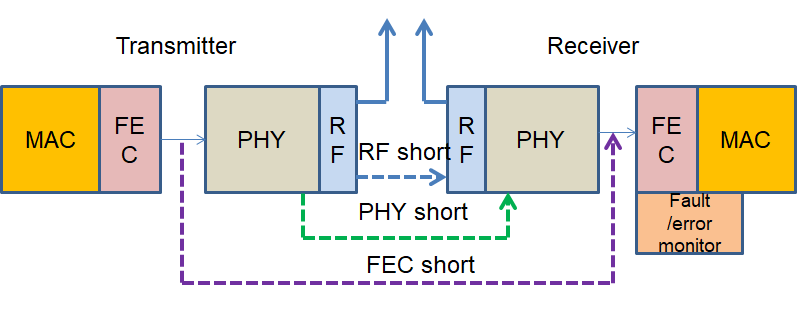
\includegraphics[width=0.65\textwidth]{figures/Shorts.png}
\caption{Transmitter and receiver shortcut idea for diagnostic test purposes}
\label{fig:Shorts}
\end{figure}

In order to conduct such test, the physical shorts need to be implemented. A simple multplexer demultiplexer pair with the common control logic would allow to choose between a normal functionality and shortened path. Additionally the test vectors need to be generated or stored in ROM. A good alternative would also be to do a "fake" start-up to detect all errors that may prevent the synchronization in advance. The test may be followed by random test to uncover other faults. The generation can happen even in software and be sent as normal information over the channel. The fault detection occurs thanks to an extended decoder functionality, which signalizes, with a special ISERR output, if the current bit of the bit stream has been flipped or not. This functionality is intended also to be used during the normal data flow, to adjust the transmission parameters and adapt the FEC algorithm. A simple counter connected to this special output counts the number of bit flips in every block. This information can be used for channel quality estimation, since the more errors per message, the worse is the transmission channel quality. 

The idea of functional shorts has been implemented into the Test Bench together with error injection capability and is shown in \autoref{fig:short_ena}. The injected error vector travels through the design together with test data. This guaranties the proper alignment of the error vector with the test vector at any time, also during the shortcut, when the path is shorter. It flips the specified bits of the output of any chosen module to simulate the possible effects of hardware faults on the processed information. The implementation lacks real modules, except for the encoder and decoder. Every other module is implemented as a simple delay in the digital information flow (flip flop) and XOR gate to conduct the error injection. They also have special enable signal to choose which module should occur as faulty. The enable signal is exclusive, meaning that only one module may be faulty at the same time. The Air simulates the communication channel. There is also a programmable delay to variate the execution time of the test and to simulate the fact, that the number of clock cycles, needed for the information to pass from the encoder to decoder, is not constant in all tests.

\begin{figure}[h]
\centering
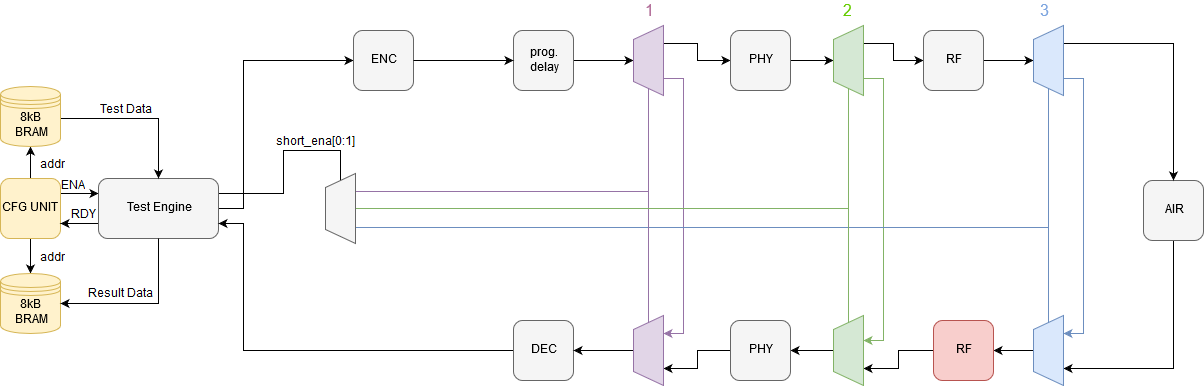
\includegraphics[width=\textwidth]{figures/Short_ena_err.png}
\caption{Implementation of functional shorts into the Test Bench}
\label{fig:short_ena}
\end{figure}

\subsection{Diagnostic test Procedure}
Let's assume, that the FEC decoder is fault-free and that every module owns some sort of repair ability. The erroneous unit would be the Radio Frequency unit of the receiver (marked red in \autoref{fig:short_ena}).
\begin{enumerate}
    \item Start the test by enabling the shortcut nr. 3, closing the test loop between transmitter and receiver, excluding all transmission errors from the test.
    \item Conduct the test by running all test vectors through the design, placing them on the inputs of FEC encoder, until the first occurrence of the ISERR output of the decoder module.
    \item Enable Shortcut nr. 2.
    \item Run test again and detect no errors, since the faulty unit is not in the test loop.
    \item Run repair procedure on the transmitter RF unit.
    \item Enable Shortcut nr. 3.
    \item Run the test only to see the ISERR is high again, because the repaired unit was not the faulty one.
    \item Run repair procedure on RF unit of the receiver, revert the repair of the transmitter RF unit.
    \item Start the test again to see no errors detected.
    \item Log the information about the repaired unit.
    \item Switch off all Shortcuts and start normal operation.
\end{enumerate}

After running the tests, all injected errors have been detected and the shorts system was able to identify the faulty unit. The number of injected faults have deliberately never exceeded the error correction capabilities of the decoder and the decoder was always assumed to be fault-free. Additionally the faults have been injected in random places, not necessarily corresponding to real permanent faults effects. Since the encoder and decoder are the only real modules in the test loop and their fault free functionality is crucial to the successful diagnostic test, they have been tested in isolated environment to understand their behavior and test their limits and possible impact on the whole system.